% !TeX spellcheck = cs_CZ
%{\tikzset{external/prefix={tikz/FYZII/}}
% \tikzset{external/figure name/.add={ch24_}{}}
%---------------------------------------------------------------------------------------------------
% file fey2ch24.tex
%---------------------------------------------------------------------------------------------------
%=========================== Kapitola Vlnovody =====================================================
\setchaptertoc
\chapter{Vlnovody}\label{fyz:IIchapXXIV}

  \section{Přenosové vedení}\label{fyz:IIchapXXIVsecI}
  \section{Obdélníkový vlnovod}\label{fyz:IIchapXXIVsecII}
  \section{Mezní frekvence}\label{fyz:IIchapXXIVsecIII}
  \section{Rychlost šíření vln ve vlnovodu}\label{fyz:IIchapXXIVsecIV}
  \section{Detekování vedených vln}\label{fyz:IIchapXXIVsecV}
  \section{Spojování vlnovodů}\label{fyz:IIchapXXIVsecVI}
  \section{Mody vlnovodů}\label{fyz:IIchapXXIVsecVII}
  \section{Jiný pohled na vlnovody}\label{fyz:IIchapXXIVsecVIII}
  \section{Příklady a cvičení}\label{fyz:IIchapXXIVsecIX}

    \begin{figure}[ht!] %\ref{fyz:fig0559}
      \centering
      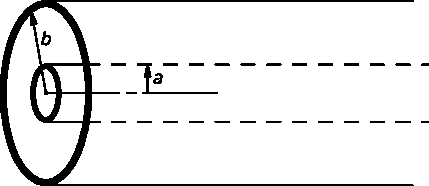
\includegraphics[width=0.7\linewidth]{fyz_fig0559.pdf}
      \caption{
               (\cite[s.~707]{Feynman02})}
      \label{fyz:fig0559}
    \end{figure}

    \begin{figure}[ht!] %\ref{fyz:fig0560}
      \centering
      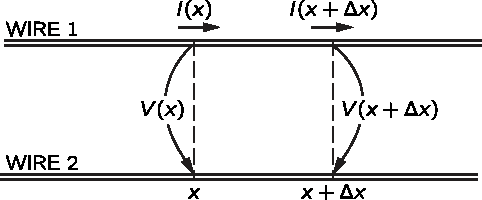
\includegraphics[width=0.7\linewidth]{fyz_fig0560.pdf}
      \caption{
               (\cite[s.~707]{Feynman02})}
      \label{fyz:fig0560}
    \end{figure}

    \begin{figure}[ht!] %\ref{fyz:fig0561}
      \centering
      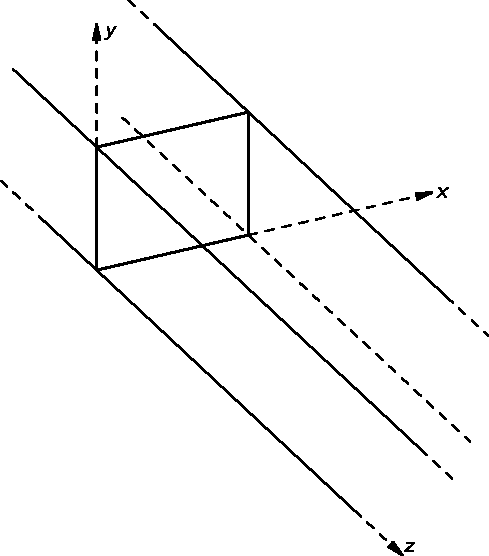
\includegraphics[width=0.7\linewidth]{fyz_fig0561.pdf}
      \caption{
               (\cite[s.~707]{Feynman02})}
      \label{fyz:fig0561}
    \end{figure}

    \begin{figure}[ht!] %\ref{fyz:fig0562}
      \centering
      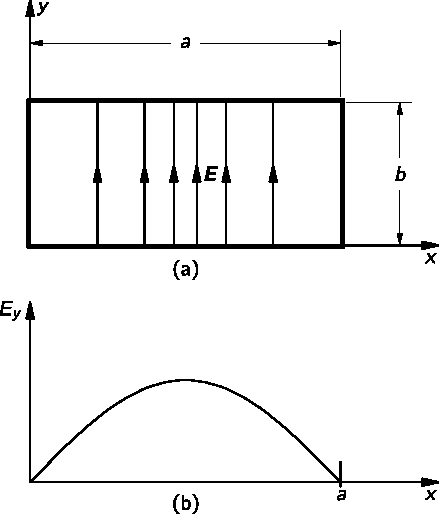
\includegraphics[width=0.7\linewidth]{fyz_fig0562.pdf}
      \caption{
               (\cite[s.~707]{Feynman02})}
      \label{fyz:fig0562}
    \end{figure}

    \begin{figure}[ht!] %\ref{fyz:fig0563}
      \centering
      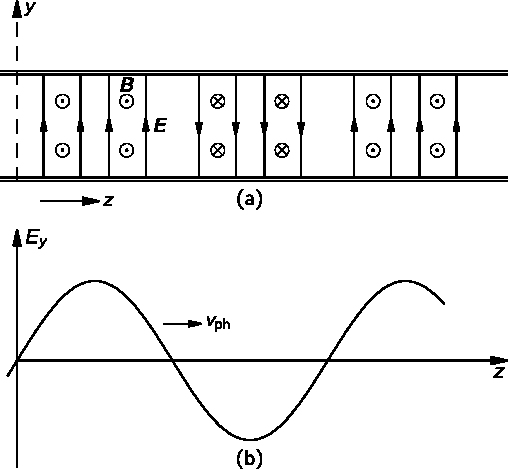
\includegraphics[width=0.7\linewidth]{fyz_fig0563.pdf}
      \caption{
               (\cite[s.~707]{Feynman02})}
      \label{fyz:fig0563}
    \end{figure}

    \begin{figure}[ht!] %\ref{fyz:fig0564}
      \centering
      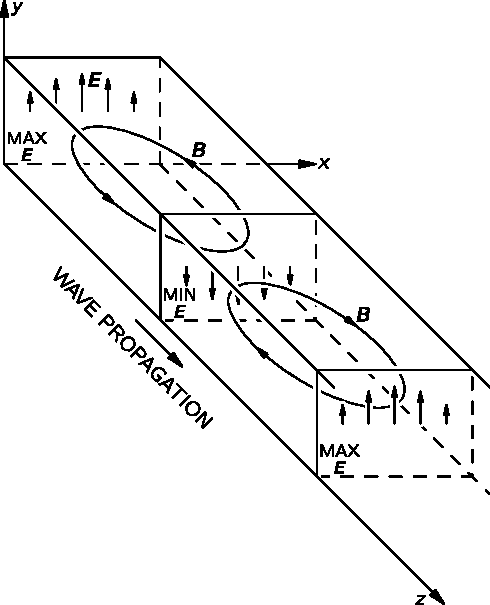
\includegraphics[width=0.7\linewidth]{fyz_fig0564.pdf}
      \caption{
               (\cite[s.~707]{Feynman02})}
      \label{fyz:fig0564}
    \end{figure}

    \begin{figure}[ht!] %\ref{fyz:fig0565}
      \centering
      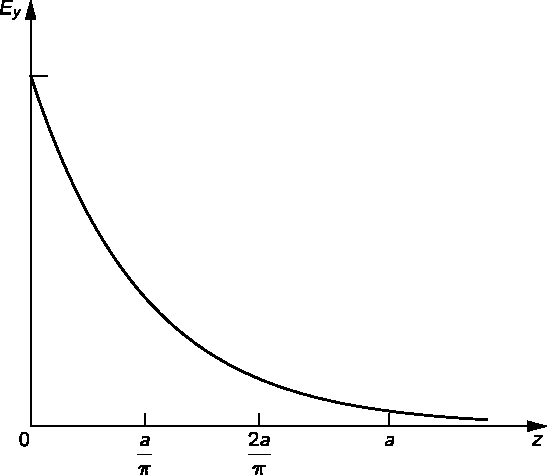
\includegraphics[width=0.7\linewidth]{fyz_fig0565.pdf}
      \caption{
               (\cite[s.~707]{Feynman02})}
      \label{fyz:fig0565}
    \end{figure}

    \begin{figure}[ht!] %\ref{fyz:fig0566}
      \centering
      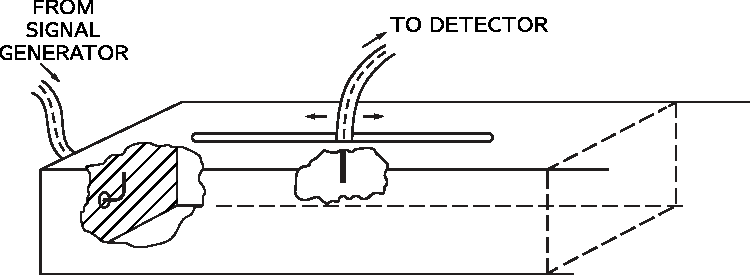
\includegraphics[width=0.7\linewidth]{fyz_fig0566.pdf}
      \caption{
               (\cite[s.~707]{Feynman02})}
      \label{fyz:fig0566}
    \end{figure}

    \begin{figure}[ht!] %\ref{fyz:fig0567}
      \centering
      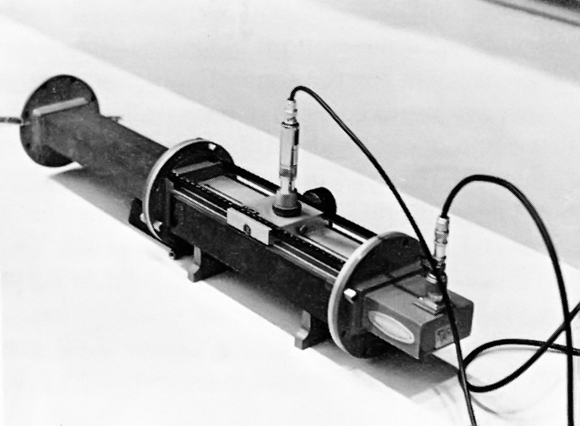
\includegraphics[width=0.7\linewidth]{fyz_fig0567.jpg}
      \caption{
               (\cite[s.~707]{Feynman02})}
      \label{fyz:fig0567}
    \end{figure}

    \begin{figure}[ht!] %\ref{fyz:fig0568}
      \centering
      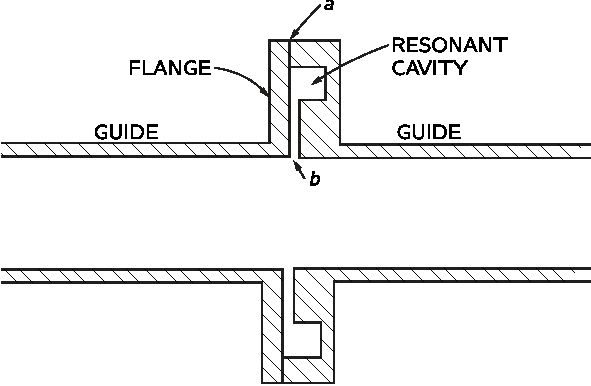
\includegraphics[width=0.7\linewidth]{fyz_fig0568.pdf}
      \caption{
               (\cite[s.~707]{Feynman02})}
      \label{fyz:fig0568}
    \end{figure}

    \begin{figure}[ht!] %\ref{fyz:fig0569}
      \centering
      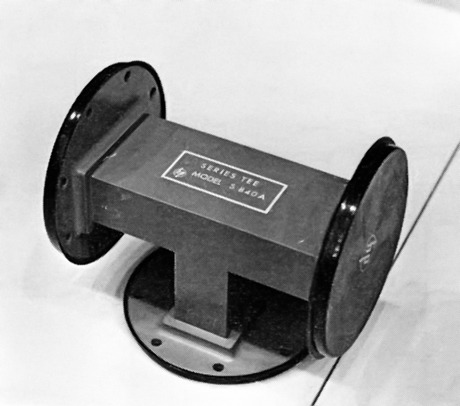
\includegraphics[width=0.7\linewidth]{fyz_fig0569.jpg}
      \caption{
               (\cite[s.~707]{Feynman02})}
      \label{fyz:fig0569}
    \end{figure}

    \begin{figure}[ht!] %\ref{fyz:fig0570}
      \centering
      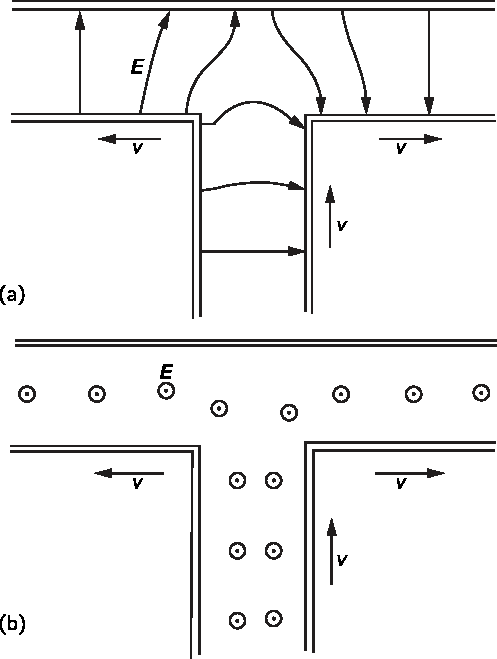
\includegraphics[width=0.7\linewidth]{fyz_fig0570.pdf}
      \caption{
               (\cite[s.~707]{Feynman02})}
      \label{fyz:fig0570}
    \end{figure}

    \begin{figure}[ht!] %\ref{fyz:fig0571}
      \centering
      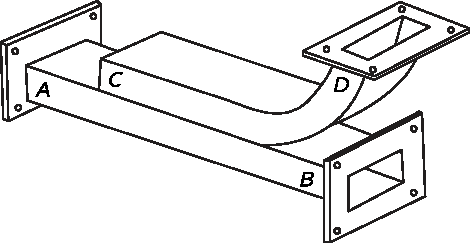
\includegraphics[width=0.7\linewidth]{fyz_fig0571.pdf}
      \caption{
               (\cite[s.~707]{Feynman02})}
      \label{fyz:fig0571}
    \end{figure}

    \todo[inline]{Kapitola fey2ch24 je nedodělaná, obsahuje pouze obrázky}
%} %tikzset
%---------------------------------------------------------------------------------------------------
